% !TEX root = ../thesis-example.tex
%
\chapter{Robot Simulation}
\label{sec:robotics-simulation}

\cleanchapterquote{Learning by doing, peer-to-peer teaching, and computer simulation are all part of the same equation.}{Nicholas Negroponte}{}
\let\thefootnote\relax\footnotetext{This chapter is based on the work published in \cite{MESAS:MingoHoffman:14} and revised in \cite{Springer:MingoHoffman:14}}


In this chapter, a set of plugins for Gazebo are presented. These plugins enables the interoperability of YARP modules between a real robot and a simulated one. Gazebo is an open-source simulation environment developed by the Open Source Robotics Foundation. It is widely used in the robotics community thanks to its ease of use and versatility.

Since these plugins conform with the YARP layer used on the real robots, applications, written for COMAN and WALK-MAN for example, can be tested and developed also on the simulated robots with no changes. The plugins consists in two main components: a YARP interface with the same API as the real robot interface, and a Gazebo plugin which handles simulated joints, encoders, IMUs, force/torque sensors, synchronization and so on.
Different modules and tasks for COMAN and WALK-MAN have been developed using Gazebo and the presented plugins as a testbed before moving to the real robots.

This chapter is organized in the following sections: \hyperref[sec:robotics-simulation:introduction]{\textbf{introduction}}, \hyperref[sec:robotics-simulation:related-works]{\textbf{related works}}, discusses some of the most popular simulation environments in robotics, \hyperref[sec:robotics-simulation:structure]{\textbf{structure}} introduces in detail some of the Gazebo plugins developed in this work and \hyperref[sec:robotics-simulation:conclusions]{\textbf{conclusions}} summarize the outcome of this effort.

\section{Introduction}
\label{sec:robotics-simulation:introduction}
In the past years, robotics researchers have been developing many robotics frameworks such as OpenRDK \cite{Calisi:08}, YARP \cite{Metta:YARP:2006} or ROS \cite{Quigley:09} in order to ease the creation of generic applications for robots and encourage code reuse. The performance overhead introduced by these frameworks is balanced by the architectural benefits, for example they allow to build modular systems to execute one or more assigned tasks.

In these frameworks, the \emph{simulator} is a module that represents the real robot at the interface level. Such simulator module accepts control input (desired joint torques, desired joint position, ...) and outputs sensory feedback (cameras, joint positions, ...) from the simulated world. The most important aspect is that they allow to develop and test modules that directly will work in the real robot without any need to rewrite code. In fact, when the real robot is used, there is a module that replaces the simulator by providing the same hardware interfaces. For instance, a module 'A' write desired joint position and read actual joint position without knowing if it is interfaced with the simulator (Figure \ref{yarp_simulation_a}) or the real hardware (Figure \ref{yarp_simulation_b}) since they expose the same interface.
\begin{figure}
\centering
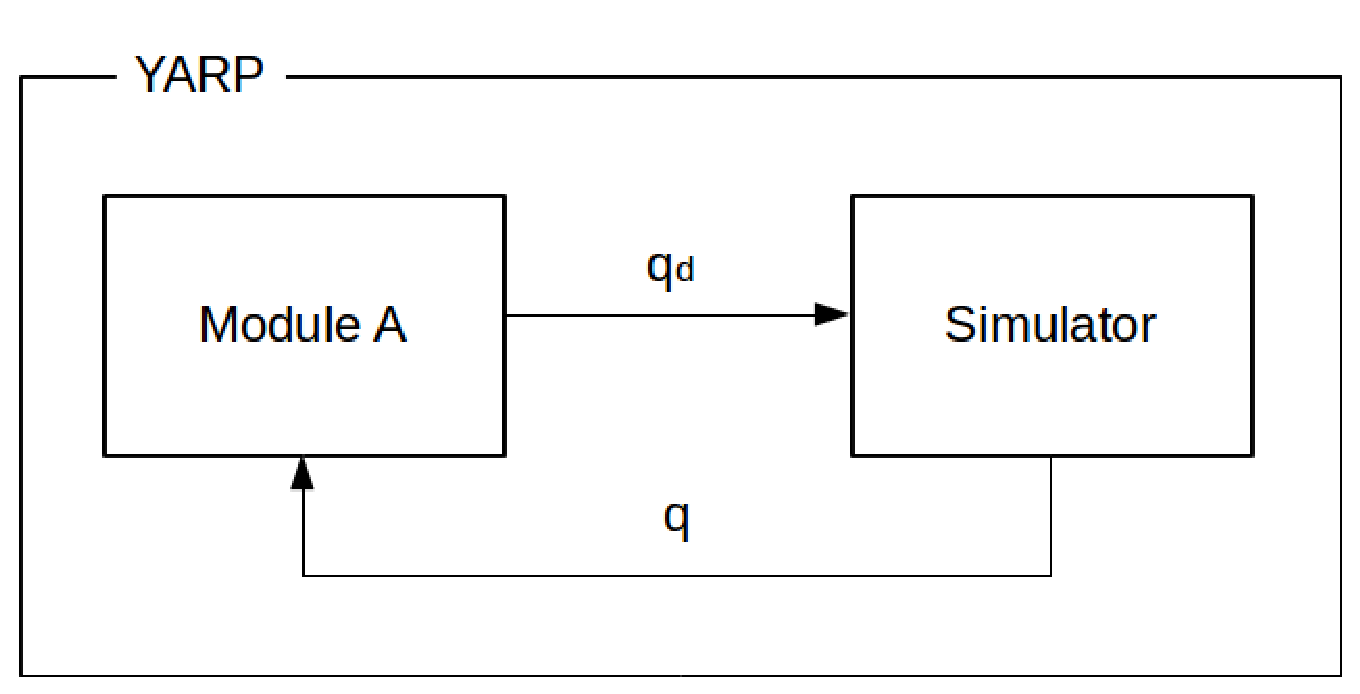
\includegraphics[height=3.5cm]{gfx/yarp_simulation_a.eps}
\caption{Module A connected to the simulator}
\label{yarp_simulation_a}
\end{figure}

\begin{figure}
\centering
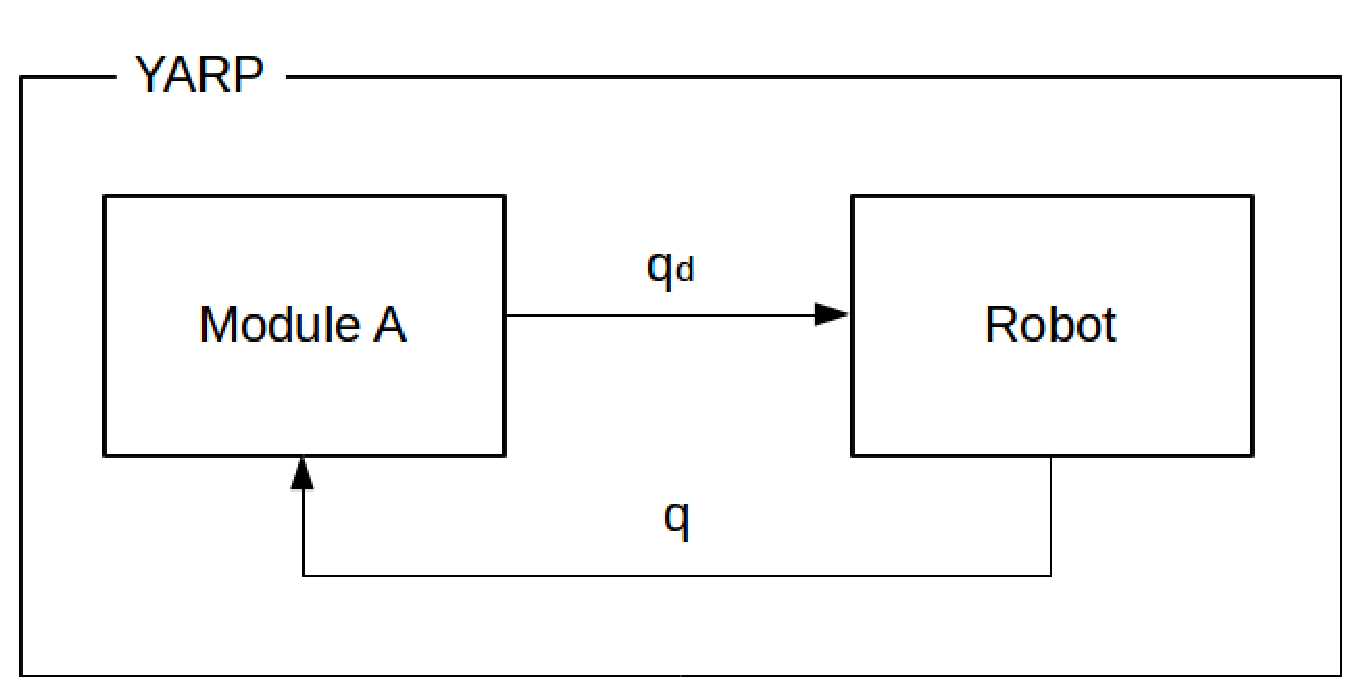
\includegraphics[height=3.5cm]{gfx/yarp_simulation_b.eps}
\caption{Module A connected to the robot}
\label{yarp_simulation_b}
\end{figure}

By accurately simulating robots and environments, code designed to operate on a real robot can be executed and validated on the simulated equivalent system. This avoids common problems associated with hardware such as short battery life, hardware failures, and unexpected and dangerous behaviors, particularly during the initial stages of development and tuning of new modules and controllers. 
It is also much faster to have a simulation engine up and running than using a real robot, especially when the simulation engine can run faster than real-time. In this way the simulator becomes a fundamental part of the framework and the robot software development cycle as the first step to validate algorithms, thus minimizing the risks of hardware breaks. 

\begin{figure}
\centering
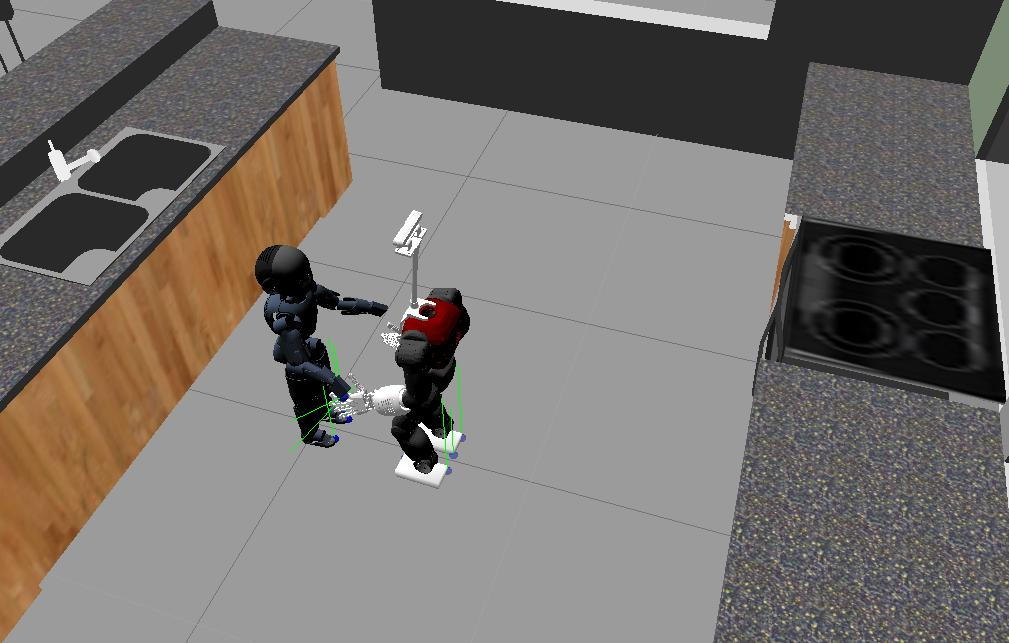
\includegraphics[height=6.5cm]{gfx/coman_icub_gazebo.jpg}
\caption{COMAN and iCub interacting inside a Gazebo simulation of a kitchen, blue dots represent contact points}
\label{coman_icub_gazebo}
\end{figure}

With these concepts in mind, in this thesis is presented an extension to one of the most known robotics simulator, Gazebo \cite{koenig2004design}, to be compatible with one of the most used robotics framework, YARP (Figure \ref{coman_icub_gazebo}), developed in the Italian Institute of Technology. 
YARP is supported by the iCub simulator (iCubSim, \cite{Tikhanoff:2008}) that is dedicated to a specific platform so the needs of a more generic tool for simulating different robots rise up. 
Gazebo, that was chosen as the simulator for the DARPA Virtual Robotic Challenge (VRC, \cite{DRC:13}), allows the use of different dynamic engines, it is easily expandable through plugins and it has a strong and active community. Gazebo is maintained by the Open Source Robotics Foundation \cite{OSRF:11}.

\section{Related Works}
\label{sec:robotics-simulation:related-works}
A large number of simulators  have been developed in the past two decades \cite{Ivaldi:14}. Such simulators range from dynamic solver libraries to complex simulation environments/systems. The latter are usually large projects that provide both rigid body dynamic simulations and tools such as graphical editors, planner libraries, visualization tools, controllers and so on. Here we want to introduce some of them, the most used by the robotics community.

The \textbf{Open Dynamics Engine} (ODE, \cite{Russel:00}) is one of the most widely used rigid body dynamics engine in robotics simulation. ODE simulates chains of rigid bodies connected and constrained by different types of joints. It has a built-in collision detection system and implements hard contacts using non-penetration constraint whenever two bodies collide. Beside the large number of project that use it, at the moment the development has been paused. 

\textbf{Bullet} \cite{Coumans:03} is another dynamic engine that implements different direct/inverse rigid body dynamic algorithms (eg. Featherstone articulated body algorithm, \cite{Featherstone:07}) as well as different solvers (eg. Mixed Linear Complementarity Problem, MLCP) and contact models. Bullet is used for a wide range of projects and its community is active and continues to improve it constantly.

\textbf{OpenRAVE} \cite{Diankov:10} provides an environment for testing, developing, and deploying motion planning algorithms in real-world robotics applications. The main focus is on simulation (the dynamic simulation based on ODE) and analysis of kinematic and geometric information related to motion planning. It provides many command line tools to work with robots and planners, and the run-time core is small enough to be used inside controllers and bigger frameworks. Industrial robotics automation is an important target application.

\textbf{Webots}  \cite{Michel:04} is a development environment used to model, program and simulate mobile robots. With Webots the user can design complex robotic setups, with one or several, similar or different robots, in a shared environment. A large choice of simulated sensors and actuators is available. The robot controllers can be programmed with the built-in IDE or with third party development environments. The robot behavior can be tested in dynamic simulated worlds (ODE based). The controller programs can optionally be transferred to commercially available real robots.

\textbf{V-REP} \cite{Rohmer:13}, similarly to Webots, embeds different tools that permit fast developing of algorithms and the code can be transferred inside real robotic hardware. It is compatible with four different dynamics engine: ODE, Bullet, Vortex \cite{VORTEX:13} (not open source) and Newton Dynamics \cite{NEWTON:13}.

\textbf{Gazebo} \cite{Koenig:04} is a multi-robot simulator for outdoor environments. As Stage (part of the Player project, \cite{Gerkey:03}), it is capable of simulating a population of robots, sensors and objects. It generates both realistic sensor feedback and physically consistent interactions between objects. It includes an accurate simulation of rigid-body physics and allows the user to select between multiple dynamics engines (ODE, Bullet, SimBody \cite{Sherman} and DART \cite{DART:13}). 

Finally, two notable softwares are the \textbf{OpenHRP} project used mostly in Japan for the HRP robot series \cite{Kanehiro:04} and \textbf{MuJoCo} \cite{Todorov:12} used mostly for model predictive control.

The decision to add a YARP interface to Gazebo is motivated by the following considerations.
The possibility to switch between fast, not accurate simulations and slow, accurate ones, thus the capability of choosing among different dynamic engines was needed. A simulator which is both easy to use and to expand in order to add new robot models, sensors and so on. Finally, the preference of open-source software with an active community and money investments.
Gazebo fulfills all the requirements, in particular it is expandable with a plugin structure: in this work the YARP interface is a collection of Gazebo plugins. 


\section{Structure}
\label{sec:robotics-simulation:structure}
It is useful to understand Gazebo plugins and YARP device drivers before describing the structure of the plugins developed in this work (from now on \textbf{gazebo\_yarp\_plugins}).

Gazebo plugins are C++ classes that extend the functionalities of Gazebo, while YARP device drivers are C++ classes used in YARP for abstracting the functionality of robot devices.
Usually, each class of gazebo\_yarp\_plugins embeds a YARP device driver in a Gazebo plugin. 

\subsection{Gazebo Plugins}
A plugin is a piece of code compiled as a shared library and inserted into the simulator. A plugin has direct access to all the functionalities of Gazebo from the physics engine to the simulated world. Furthermore, plugins are self-contained routines that are easily shared and can be inserted and removed from a running system. There are 5 types of plugins in Gazebo: \textbf{world}, \textbf{model}, \textbf{sensor} plugins are attached to and control a specific simulated world/model/sensor respectively, a \textbf{system} plugin is specified on the command line and loads during the Gazebo startup and finally a \textbf{visual} plugin can be used to display informations during the simulation.


\subsection{YARP Device Drivers}
YARP provides special devices that act as network proxies and make interfaces available through a network connection. This allows accessing devices remotely across the network without code change.

A device driver is a class that implements one or more interfaces. There are three separate concerns related to devices in YARP:
\begin{itemize}
\item Implementing specific drivers for particular devices
\item Defining interfaces for device families
\item Implementing network wrappers for interfaces
\end{itemize}
For example the Control Board device driver implements a set of interfaces that are used to control the robot (IPositionControl, ITorqueControl, etc.) and another set of interfaces to read data from the motors (IEncoders, etc).

\subsection{Gazebo-YARP Plugins}
A gazebo\_yarp\_plugins is made of:
\begin{itemize}
    \item Gazebo plugins that instantiate YARP device drivers,
    \item YARP device drivers that wrap Gazebo functionalities inside the YARP device interfaces.
\end{itemize}
Some examples of implemented plugins are the \textbf{Control Board}, \textbf{6-axis Force Torque sensor}, \textbf{Inertial Measurement Unit} (IMU) and the \textbf{Clock} plugin used for synchronization.
The first three plugins are directly related to the simulated objects and sensors, while the last one is a system plugin that synchronizes all the other YARP modules with the simulation time. 

The \textbf{Control Board} plugin allows to control the robot using YARP Interfaces, it is implemented as a Gazebo Model plugin. Every control board allows the user to control one or more joints (a kinematic chain such as the arm or leg, etc.) as specified in a configuration file. For each controlled joint, the control board opens different interfaces, permitting the use of different type of controllers for each joint. Such interfaces include position control, torque control, encoders reading, torque measurement and joint impedance control. Usually the number of instantiated control boards is equal to the number of kinematic chains. Each control board, during every cycle of simulation, reads position, velocity and torque values from the simulated joints and sends desired joints position or torques to the simulator. The values read from the simulator are then broadcasted through YARP interfaces in the YARP network, in a similar way the desired joint values come from YARP interfaces (Figure \ref{control_board}). The following YARP interfaces are used to control the robot.
\begin{itemize}
\item \textbf{IPositionControl}: a position control with a linear trajectory generator considering a max joint speed
\item \textbf{IPositionDirect}: a position control using Gazebo position PIDs
\item \textbf{ITorqueControl}: a perfect torque follower
\item \textbf{IImpedanceControl}: a joint impedance control with the following law
\begin{equation}
    \tau_d = -P_d(q-q_d) - D_d\dot{q} + \tau_{offset}
\end{equation}
where $q_d$ is the desired equilibrium position, $P_d$ is the desired joint stiffness and $D_d$ is the desired joint damping. $\tau_{offset}$ is an extra signal that can be used for gravity compensation or inverse dynamics control.
\end{itemize}
Furthermore, the Control Board implements the \textbf{IControlMode} interface that allows to change the type of controller on-line. All these interfaces are also available on the robot and they have the same behaviour.
\begin{figure}
  \centering
    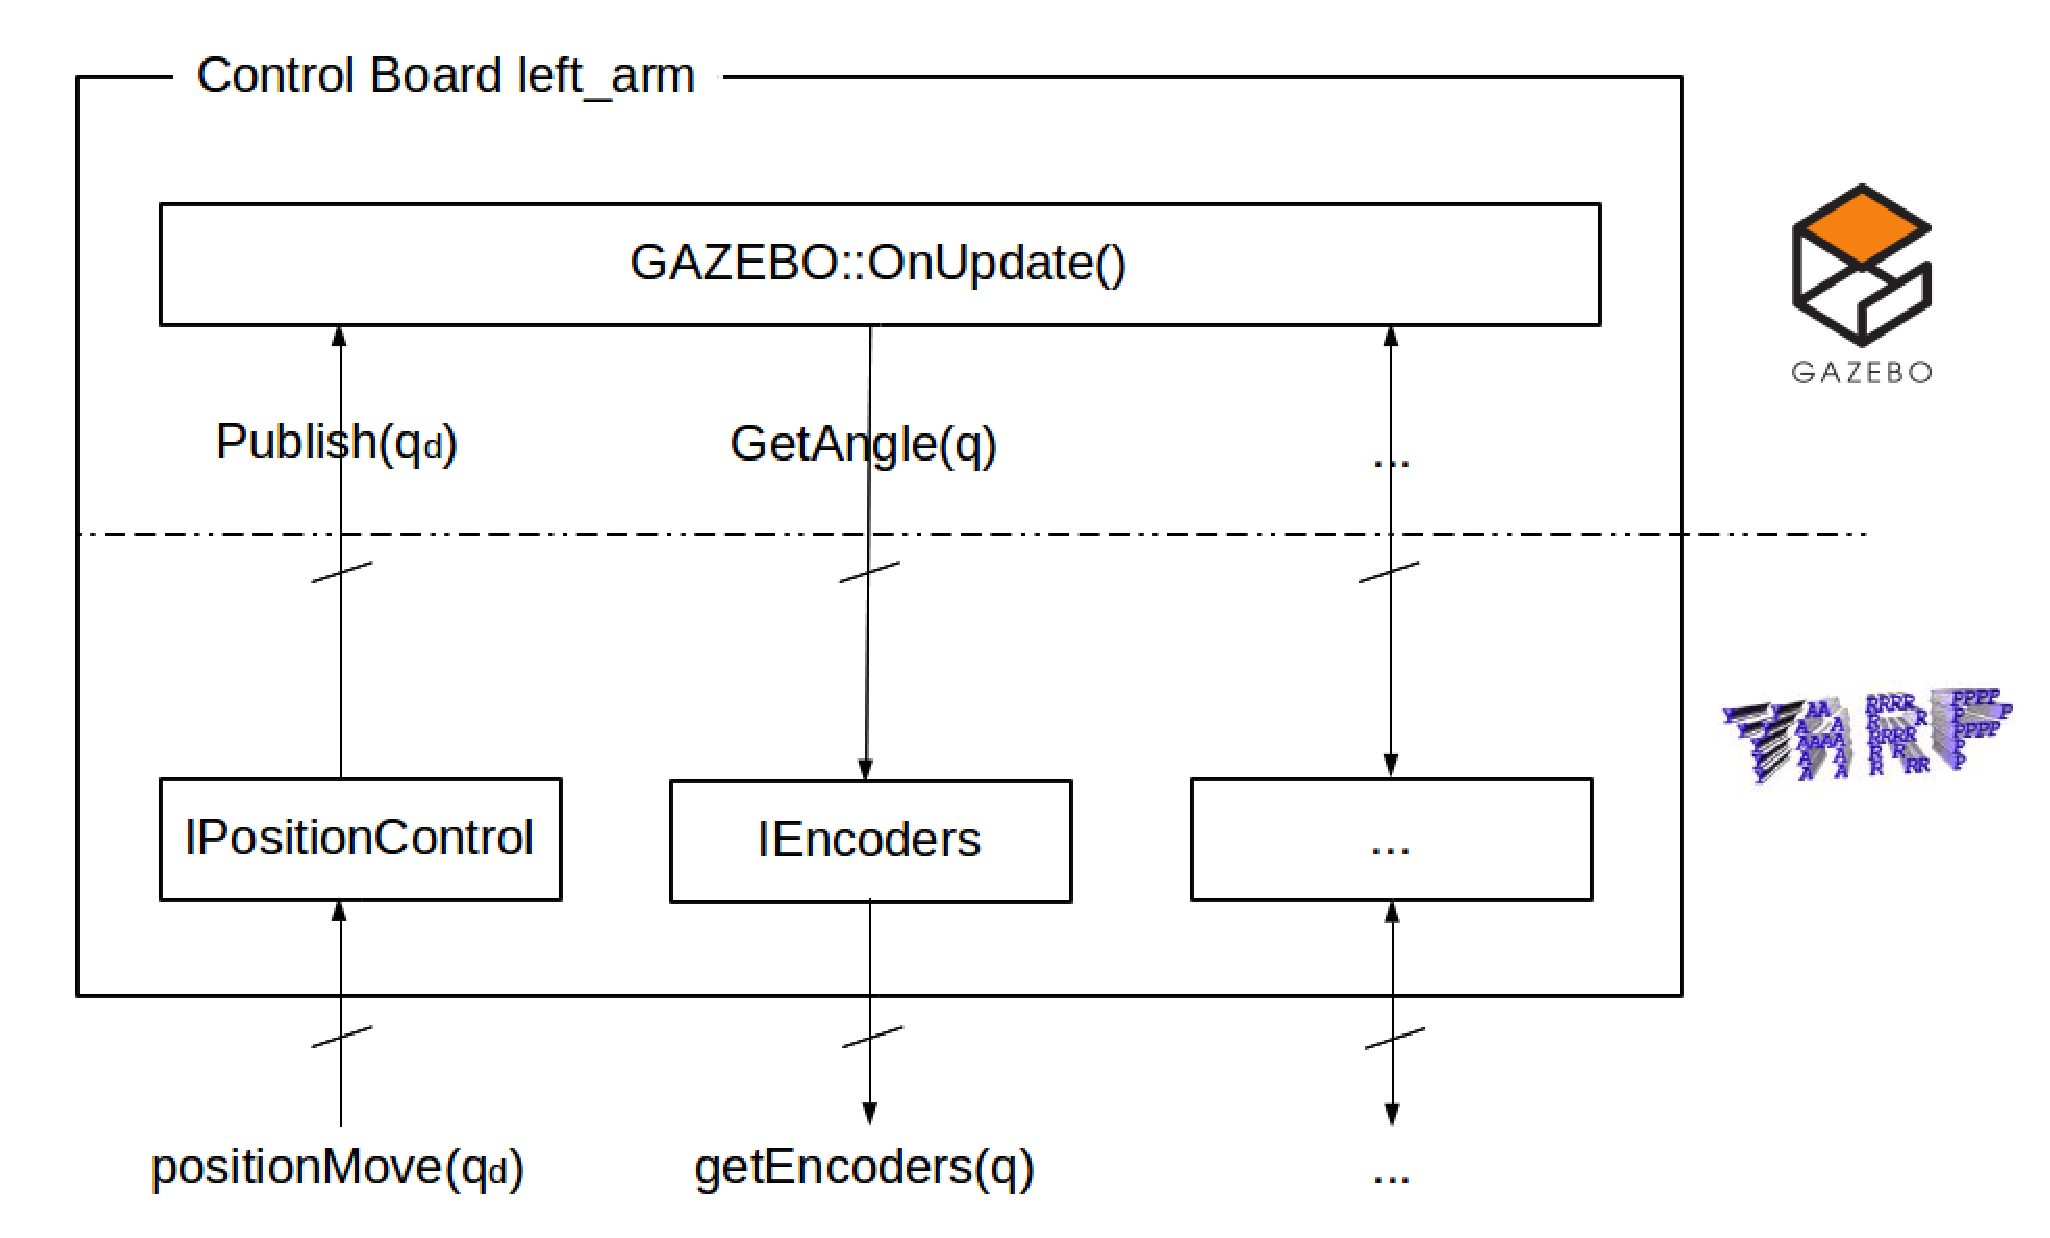
\includegraphics[height=6.5cm]{gfx/control_board.eps}
    \caption{A Control Board plugin for a kinematic chain. The yarp::IPositionControl interface has a method positionMove() that can be used to set joint values inside a YARP module. The plugin implements such interface by calling the Publish() method inside the Gazebo API to move the simulated joints at each OnUpdate()}\label{control_board}
\end{figure}


A \textbf{Force/Torque sensor} measures a wrench in the robot structure. The sensor, at the time of writing, is simulated in Gazebo as if it was attached to the reference frame associated to a joint. On the YARP side, the reading of a generic sensor is implemented as a \textbf{IAnalogSensor} interface (Figure \ref{ianalog_force_torque}). The broadcasted data is a vector of six numbers representing the forces and the torques applied on that reference frame. 
\begin{figure}
  \centering
    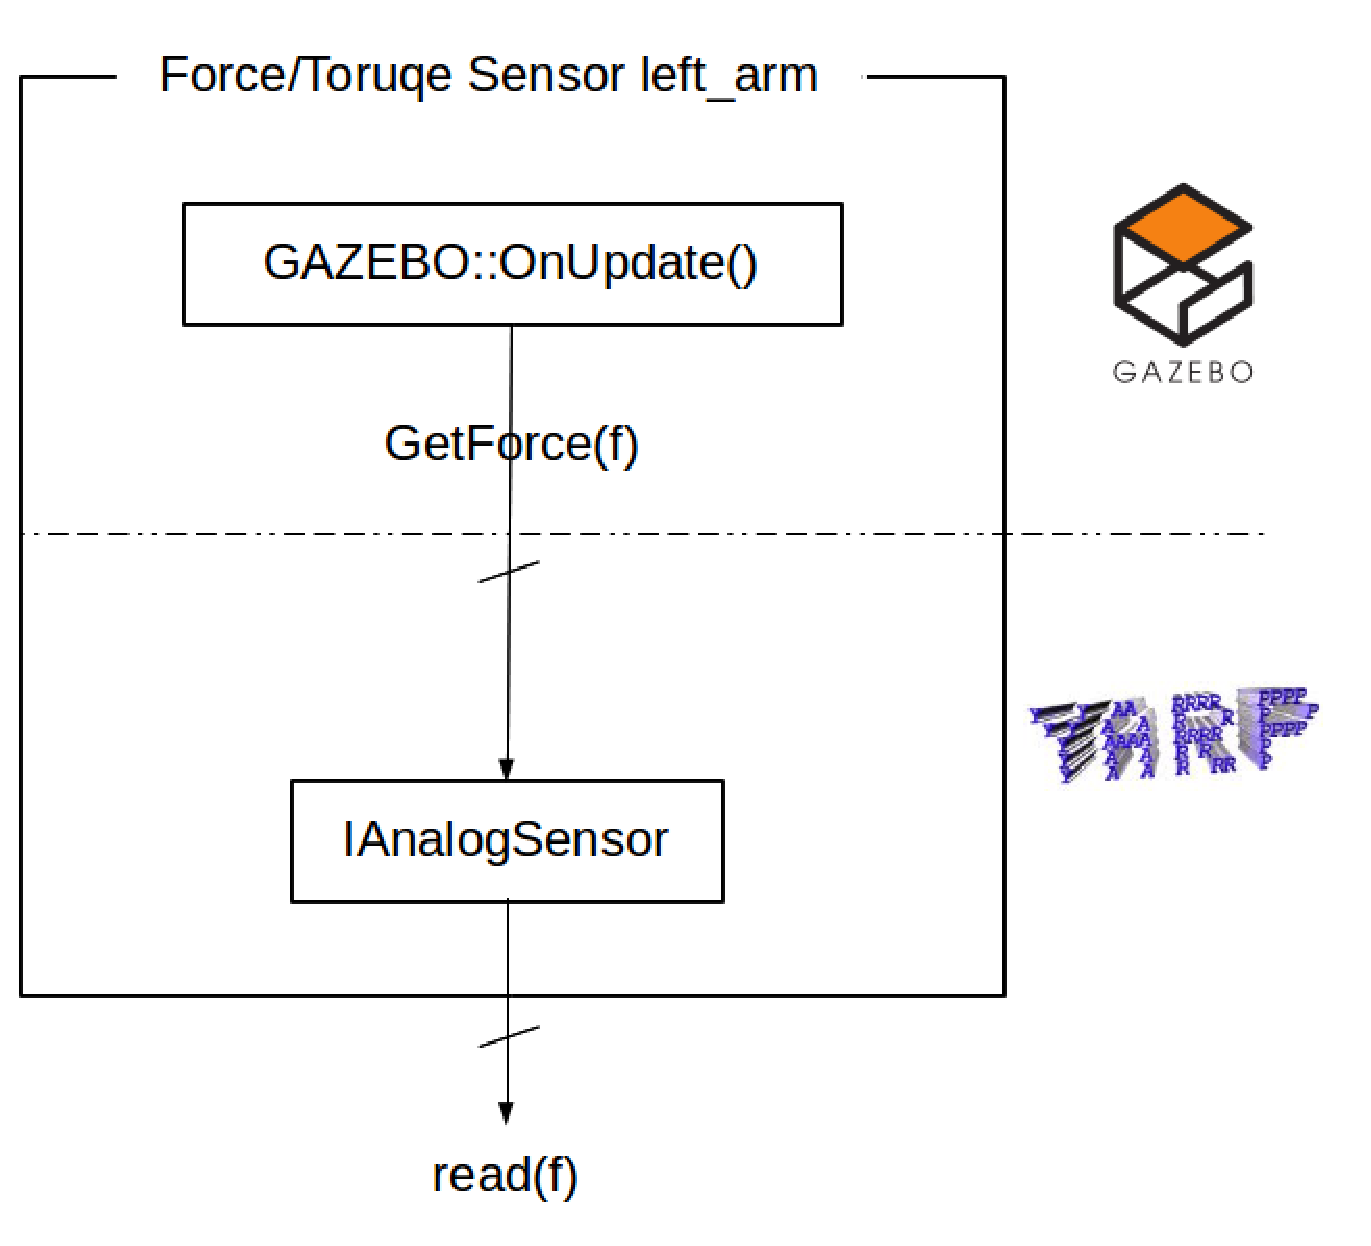
\includegraphics[height=6.5cm]{gfx/ianalog_force_torque.eps}
    \caption{The Force/Torque sensor plugin is implemented as a YARP IAnalogSensor interface. At every step the internal state of the plugin is updated with the last readings of forces and torques from the simulation}\label{ianalog_force_torque}
\end{figure}


An \textbf{IMU} measures velocity, orientation, and gravitational forces, using a combination of accelerometers and gyroscopes, of the link where it is placed. It is also possible to add white Gaussian noise on the measurement.
Similar to the Force/Torque sensor, it is implemented as a \textbf{IAnalogSensor} interface.
\begin{figure}
  \centering
    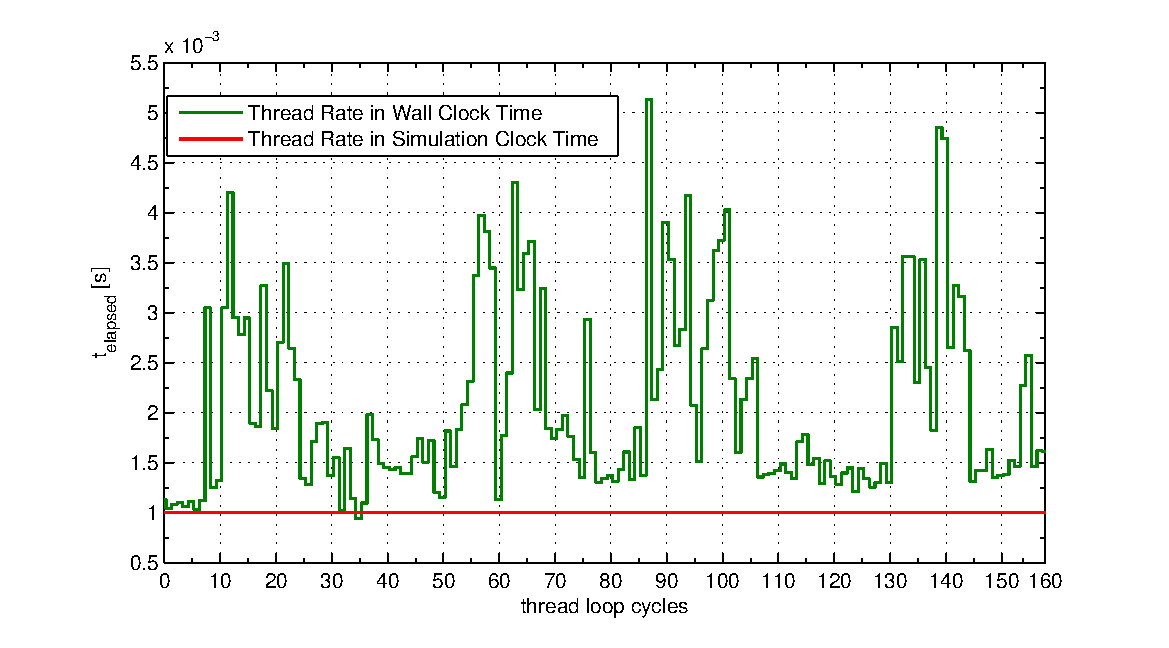
\includegraphics[height=6.5cm]{gfx/yarp_clock.eps}
    \caption{Time elapsed between each execution of the control loop, measured in simulation clock time and in wall clock time. Desired thread rate is $1$kHz and simulation time step is $1$ms}\label{yarp_clock_real_vs_simulated}
\end{figure}


A fundamental aspect in simulations is the synchronization between control modules and the simulated robot. A YARP control module is a process in which one or more threads are started. When such modules are used in the real robot, the thread rate is timed by the machine (system) clock, also called the wall clock. When the simulation is running we want the rate of such modules to be synchronized with the simulated time, otherwise the control loop could run faster or slower with respect to the simulated robot dynamics.
The real-time factor (RTF) of the simulation is given by 
\begin{equation}
    RTF = update\_frequency \times step\_time
\end{equation}
and is kept to one when the desired update frequency is the inverse of the time increased at each step in the simulation.
For instance if the simulation runs with a real time factor of 0.1, 10 seconds are needed to simulate 1 real second. Within this situation, the controller process should also be slowed down 10 times to be coherent with the simulation. To solve this issue we developed a \textbf{Clock} plugin that synchronizes modules with the simulated time.
The clock plugin is implemented as a System plugin and publishes on a YARP port the time information from the simulator. For every simulation step, the simulation time is incremented and the timestamp is sent via socket.
YARP functions that provide access to the computer internal clock and support thread scheduling can be synchronized with an external clock (this is enabled with the \texttt{YARP\_CLOCK} environment variable). YARP classes supporting periodic threads (RFModule and RateThread) are therefore automatically synchronized with the clock provided by the simulator. The \texttt{yarp::os::Time} functionalities are also transparently working using the wall-clock or the simulation clock depending on the environment variable. Thread sleeps are performed using the right wall or simulated time.
When synchronized with the simulation clock the \texttt{yarp::os::Time} delay does not explicitly sleep on a wall clock, rather a scheduler is synchronized with the simulation clock by performing blocking reads on the \texttt{YARP\_CLOCK} port. This scheduler wakes up the threads that required a delay just once, when they have slept for the desired duration. Compared to the \texttt{ROS::Time} implementation which uses small sleeps on wall clock to check synchronization with the simulated clock, this allows to run simulations both slower and faster than real time and still have synchronization between threads and controls. In any case, when accessing the simulated clock experiments showed the approach to be successful in synchronizing $1$kHz control loops against simulations running $1$kHz, thus having a $1$ms clock granularity.
A similar solution for synchronization has been consequently used also in \cite{Eljaik:14}.

\subsection{Simulation Description Format (SDF)}
Gazebo uses an XML-style format, Simulation Description Format (SDF), to save and load information about a simulated world or model. An SDF encapsulates all the necessary information for a simulation such as:
\begin{itemize}
\item \textbf{Scene}: ambient lighting, sky properties, shadows.
\item \textbf{Physics}: gravity, time step, physics engine.
\item \textbf{Models}: collection of links, collision objects, joints, and sensors.
\item \textbf{Lights}: point, spot, and directional light sources.
\item \textbf{Plugins}: world, model, sensor, and visual plugins.
\end{itemize}
The Control Board, Force Torque sensor and IMU plugins are included inside the SDF file that describes the robot. The clock plugin is loaded trough a command line parameter when the simulator is started.
\begin{figure}
  \centering
    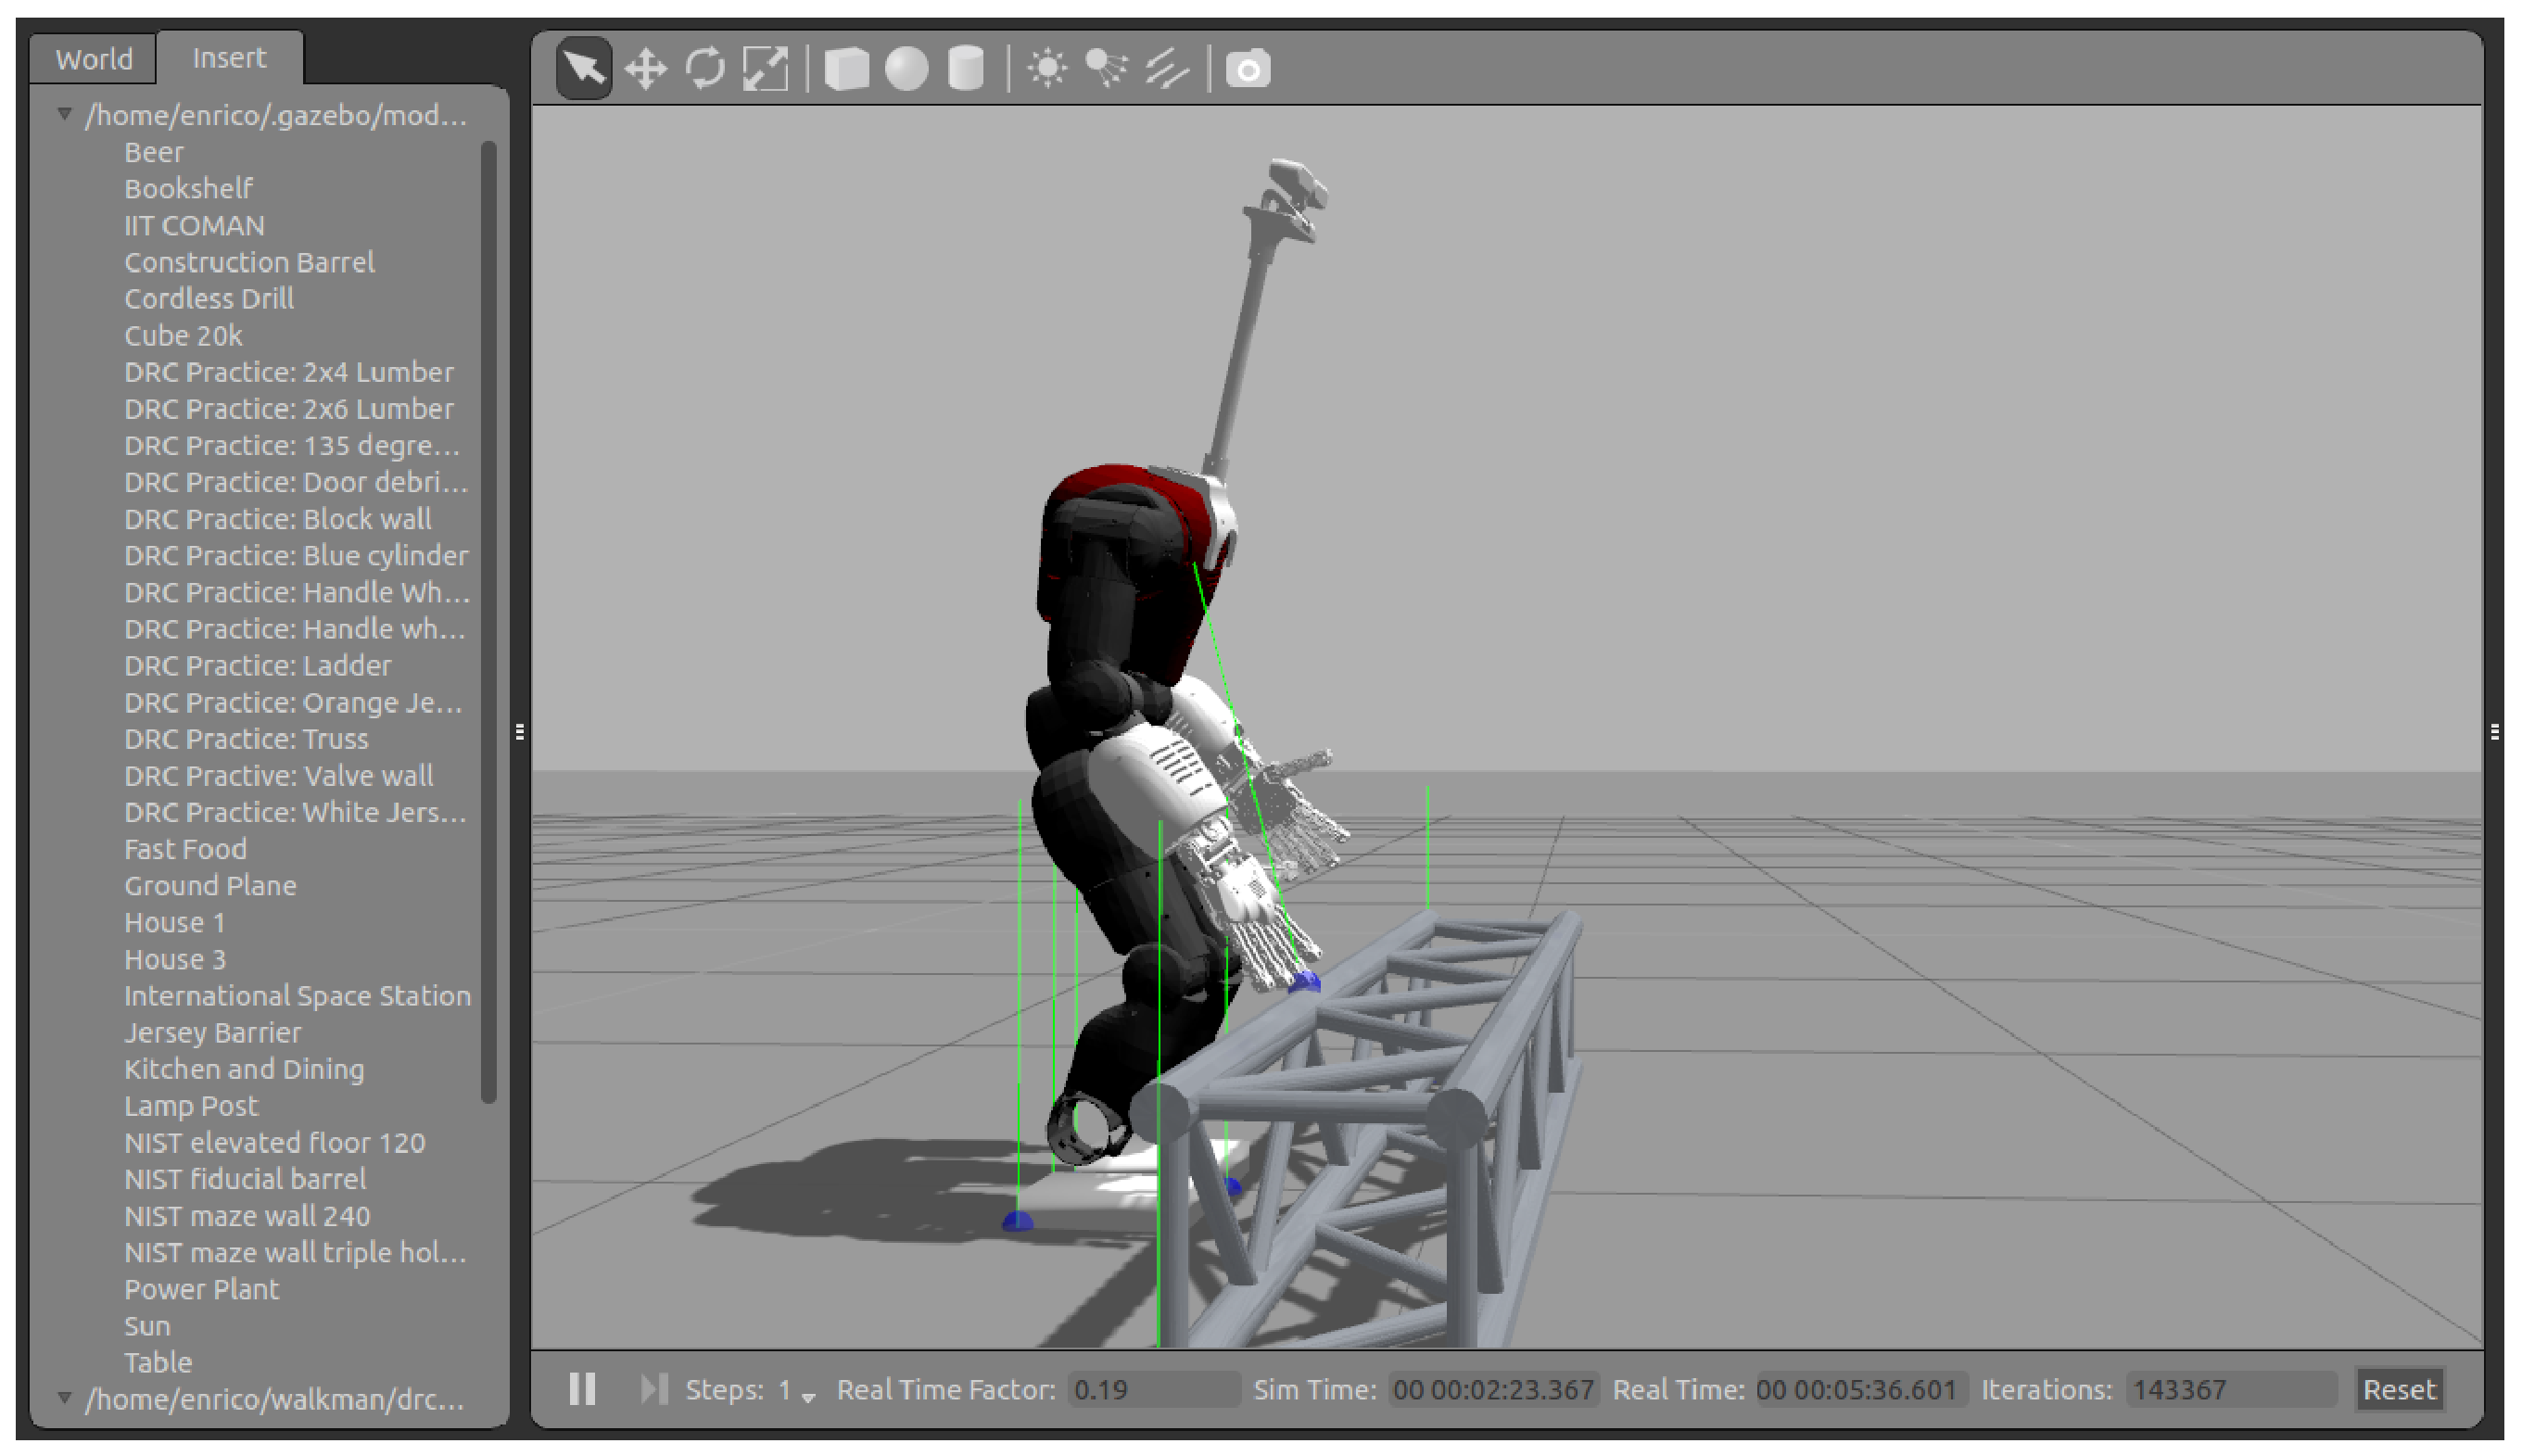
\includegraphics[height=6.5cm]{gfx/coman_ft_a.eps}
    \caption{A simulation where COMAN interact with the environment}\label{coman_ft}
\end{figure}


\section{Conclusions}
\label{sec:robotics-simulation:conclusions}
In this chapter, a set of Gazebo plugins, named \textbf{gazebo\_yarp\_plugins}, that allow to connect the robotics framework YARP to Gazebo, have been presented. Gazebo was chosen since it is easy to use, it has the possibility to switch between different dynamics engines, it is open source and it has a large active community. The gazebo\_yarp\_plugins are based on YARP device drivers in order to have exactly the same interfaces in the real and simulated robot. This allows to write modules that will work both in the simulator and in the real robot without the need to change the code: a very important paradigm in robotics research and development since it minimizes the presence of errors due to code porting. Furthermore the simulator becomes a tool that helps the developer in testing and validation before using the real platform.

As mentioned at the begging, many control modules have been designed and implemented for different humanoid platforms such as COMAN (Figure \ref{coman_ft}), iCub and WALK-MAN using these plugins. At the moment in which this thesis is written, this project is under the development of the YARP community and the source code is available at \url{https://github.com/robotology/gazebo-yarp-plugins}.
